%\PassOptionsToPackage{dvipsnames}{xcolor}
\PassOptionsToPackage{table}{xcolor} %vv important to do it this way (and not like the website says to do)!!!!
\newcommand\hmmax{0} %to deal with various fonts,e.g. mathbf
\newcommand\bmmax{0} %same
\documentclass[10pt]{beamer}

\usetheme[progressbar=frametitle]{metropolis}
\usepackage{appendixnumberbeamer}
%\setbeamersize{text margin left=5mm,text margin right=5mm} 

\usepackage{booktabs}
\usepackage[scale=2]{ccicons}

\usepackage{pgfplots}
\usepgfplotslibrary{dateplot}

\usepackage{xspace}

%\usepackage{setspace} pose problems with footnotes
\newcommand{\themename}{\textbf{\textsc{metropolis}}\xspace}

\usepackage{dashbox}
\usepackage{centernot}
\usepackage{amsmath}
\usepackage[compatibility=false]{caption}
\usepackage{wasysym}
\usepackage{fontawesome5}
\usepackage{stmaryrd}
\usepackage{marvosym}
\usepackage{subcaption}
\usepackage{multicol}
\usepackage{graphicx}
\usepackage{tabto}
\usepackage[normalem]{ulem}
\usepackage{ragged2e}
\usepackage{multirow}
\usepackage{amssymb}
\usepackage{nicefrac}
\usepackage{pifont}
\usepackage{bm}
\usepackage{cancel}
\usepackage{tikz}
\usetikzlibrary{arrows,matrix}
\usetikzlibrary {arrows.meta}
\usepackage{mathptmx}
\usepackage[style=apa, natbib, sorting=ynt]{biblatex}
\renewcommand*{\bibfont}{\scriptsize}
\addbibresource{bibliography.bib}
\usepackage{breakurl}  
\usepackage{hyperref} 
\usepackage{verbatim}

\usepackage[linguistics]{forest}
\usepackage{gb4e}

%color blind friendly
\definecolor{orange}{RGB}{213, 94, 0}
\definecolor{blue}{RGB}{0, 114, 178}
\definecolor{lightblue}{RGB}{86, 180, 233}
\definecolor{green}{RGB}{0, 158, 115}
\definecolor{red}{RGB}{204, 121, 167}
\definecolor{purple}{HTML}{9467bd}


\newcommand{\pplus}{\textcolor{orange}{$\mathbf{p^+}$}}
\newcommand{\p}{\textcolor{blue}{$\mathbf{p}$}}
\newcommand{\qplus}{\textcolor{orange}{$\mathbf{q^+}$}}
\newcommand{\q}{\textcolor{blue}{$\mathbf{q}$}}
\newcommand{\splus}{\textcolor{orange}{$\mathbf{s^+}$}}
\newcommand{\s}{\textcolor{blue}{$\mathbf{s}$}}
\renewcommand{\r}{\textcolor{red}{$\mathbf{r}$}}
\newcommand{\strong}[1]{\textbf{\textcolor{orange}{#1}}}
\newcommand{\weak}[1]{\textbf{\textcolor{blue}{#1}}}
\newcommand{\good}[1]{\textbf{\textcolor{green}{#1}}}
\newcommand{\bad}[1]{\textbf{\textcolor{red}{#1}}}
\newcommand{\cmark}{\textcolor{green}{\textbf{\ding{51}}}}%
\newcommand{\xmark}{\textcolor{red}{\textbf{\ding{55}}}}%


\newcommand{\Exists}{\textcolor{blue}{\bm{\exists}}}
\newcommand{\Sbna}{\textcolor{purple}{\bm{\tilde{\exists}}}}
\newcommand{\Forall}{\textcolor{orange}{\bm{\forall}}}

\setbeamerfont{bibliography item}{size=\footnotesize}
\setbeamerfont{bibliography entry author}{size=\footnotesize}
\setbeamerfont{bibliography entry title}{size=\footnotesize}
\setbeamerfont{bibliography entry location}{size=\footnotesize}
\setbeamerfont{bibliography entry note}{size=\footnotesize}


\setbeamerfont{footnote}{size=\scriptsize}



\resetcounteronoverlays{exx}
\setbeamercovered{transparent}

\renewcommand{\thefootnote}{\arabic{footnote}}
\renewcommand{\thempfootnote}{\arabic{mpfootnote}}

%\setbeamertemplate{caption}[numbered] % Ensures numbered captions
\let\oldcaption=\caption
\renewcommand{\caption}[1][]{\oldcaption{\centering #1}}
\newcommand{\footciteia}[1]{\footnote{\cite{#1}, i.a.}}
\newcommand{\citenp}[1]{\citeauthor{#1}, \citeyear{#1}}


\title{Exh and only don't really compete -- they just answer different questions\footnote{Many thanks to Amir Anvari, Athulya Aravind, Gennaro Chierchia, Danny Fox, Martin Hackl, Nina Haslinger, Manfred Krifka, Viola Schmitt and Raven Zhang for their advising, feedback, or input. Thanks also to the audiences of the BerlinBrnoVienna Workshop 2024, SuB29, and AC2024 for relevant feedback on related projects.  All mistakes are my own. \vspace{2mm}}}
%\titlegraphic{\includegraphics[width=2cm]{qr.png}} 

\date{May 20, 2025}
\author[shortauthor]{Adèle Hénot-Mortier (MIT)}

\institute{35th meeting of Semantics and Linguistic Theory}
%\author{Adèle Hénot-Mortier (MIT)}



\begin{document}
	\metroset{block=fill}
	
\begin{frame}{}
	\maketitle
\end{frame}
\usebackgroundtemplate{}

\begin{frame}{What can make sentences bad?}
	\begin{itemize}
		\item Sentences can be syntactically ill-formed.
	\end{itemize}
	\begin{exe}
		\ex[*]{Ed told Jo that he likes \textbf{herself}.}
	\end{exe}
	\begin{itemize}
		\item Sentences can be contradictory, or tautological.
	\end{itemize}
	\begin{exe}
		\ex 
		\begin{xlist}
			\ex[\#]{It's raining and it's \textbf{not} raining.}
			\ex[\#]{It's raining or it's \textbf{not} raining.}
		\end{xlist}	
	\end{exe}
	\begin{itemize}
		\item Sentences may out-of-the-blue contradict standard assumptions or expectations.
	\end{itemize}
	\begin{exe}
		\ex[??] {Jo will bring her alligator to the LSA.}
	\end{exe}
\end{frame}

\begin{frame}{What is oddness?}
	\begin{itemize}
		\item Sentences sometimes feel off despite being informative, and perfectly ``reasonable'' is terms of what they implicitly assume.
	\end{itemize}
	\begin{exe}
		\ex[\#] {Jo studied in Paris or in France.\\
			Conveys: Jo studied in France.}\label{ex:hd}
	\end{exe}
	\begin{itemize}
		\item Oddness seems to come from \textbf{how} information is provided, rather than from its content.
	\end{itemize}
\end{frame}


\begin{frame}{A new approach}
	\begin{itemize}
		\item In my dissertation, I capture cases that challenge standard \textsc{Redundancy}-based approaches to oddness.
		\item The central claim is that many cases of oddness can be explained by considering that \textbf{a good sentence has to be a good answer to a good question.}
		\item I formalize this longstanding intuition by proposing a compositional model of implicit questions, sensitive to the degree of specificity conveyed by sentences.
		\item Under that view, sentences are proposals to update beliefs, but also suggest ways to \textbf{hierarchically organize such beliefs}.
	\end{itemize}
\end{frame}

%\begin{frame}{Preview of the data}
%	\begin{itemize}
	%		\item Beyond (\ref{ex:hd}), oddness appears to be triggered ``at a distance'':
	%	\end{itemize}
%	\begin{exe}
	%		\ex[\#] {Jo studied in France, or studied in London or Paris.\\
		%			Conveys: Jo studied in France or London.}
	%	\end{exe}
%	\begin{itemize}
	%		\item Or to the fact it gets triggered asymmetrically, again, in tricky ways.
	%	\end{itemize}
%	\begin{exe}
	%		\ex 
	%		\begin{xlist}
		%			\ex[] {Jo studied in France, or if not in France, in Belgium.}
		%			\ex[\#] {Jo studied in France, or if not in Belgium, in France.}
		%		\end{xlist}
	%		\ex
	%		\begin{xlist}
		%			\ex[] {If Jo studied in France, he did not study in Paris.}
		%			\ex[\#] {If Jo did not study in Paris, he studied in France.}
		%		\end{xlist}
	%	\end{exe}
%\end{frame}



%\begin{frame}{A Bizarre Adventure into Pragmatic Oddness}
\begin{frame}{Roadmap}
	\begin{enumerate}
		\item Define how implicit questions are compositionally evoked by assertions, and show why this is an independent desideratum.
		\item Capture three structurally and truth-conditionally similar sentences, which display different degrees of oddness, and as such challenge \textsc{Redundancy}-based approaches.
		\item Sketch how this can be extended to capture other cases discussed in the dissertation.
		\item Discuss how implicit questions could help outside the domain of prototypically ``redundant'' sentences (looking beyond the dissertation).
	\end{enumerate}
\end{frame}

%\usebackgroundtemplate%
%{%
	%	\includegraphics[height=\paperwidth]{./lisalisa\_transparent.png}%
	%}
\begin{frame}
	\section[Odd assertions and odd questions]{Odd assertions and odd questions}
\end{frame}

\usebackgroundtemplate{}

%\begin{frame}{Back to Redundancy}
%	\begin{itemize}
	%		\item The simplest \textsc{Redundancy}-based approach to oddness deems a sentence odd, if it is contextually equivalent to one of its simplifications.
	%	\end{itemize}
%	\begin{exe}
	%		\ex {An LF $X$ is odd if $\exists S. \ \llbracket X \rrbracket$ $\equiv$ $\llbracket S(X) \rrbracket$, with $S$ a constituent-to-subconstituent substitution operation.}
	%	\end{exe}
%	\begin{itemize}
	%		\item More complex variants of \textsc{Redundancy} almost always stick an extra function in the above definition.
	%	\end{itemize}
%	\begin{exe}
	%		\ex {An LF $X$ is odd if $\exists \langle f, S\rangle. \  \llbracket f(X) \rrbracket$ $\equiv$ $\llbracket S(f(X)) \rrbracket$, with $S$ a constituent-to-subconstituent substitution operation and $f$ an operation on LFs (e.g. subconstituent extraction).}
	%	\end{exe}
%	\begin{itemize}
	%		\item In any case, these approaches play with the structure of the LF, and its meaning, potentially at the local level.
	%	\end{itemize}
%\end{frame}
\begin{frame}{Assertions and questions}
	\begin{itemize}
		\item Assertions typically denotes propositions (sets of worlds), questions sets of propositions.
		\item Assertions update the set of our shared beliefs (the \textbf{Context Set}, a ``big'' set of worlds), by intersection.
		\item Questions partition the Context Set into cells.
	\end{itemize}
\end{frame}
\begin{frame}{Standard question semantics}
	\begin{itemize}
		\item Questions have been traditionally understood as the set of their possible answers, i.e. as relevant alternatives.
	\end{itemize}
	\begin{exe}
		\ex {$\llbracket$Who did the readings?$\rrbracket$ = $\lbrace$Jo, Ed, Al, Jo+Ed, Jo+Al ...$\rbrace$}
	\end{exe}
	\begin{itemize}
		\item Alternatives are not necessarily exclusive: if Jo and Al did the readings, then Jo did.
		\item Alternatives are ``congruent'' with the question in the following sense.
	\end{itemize}
	\begin{exe}
		\ex {\textsc{Question-Answer Congruence.} An answer to a question can be derived from it by replacing the \textit{wh}-word with a relevant alternative of suitable type.}\label{ex:qa-congruence}
	\end{exe}
\end{frame}

\begin{frame}{Standard question pragmatics}
	\begin{itemize}
		\item A conversation's Context Set (\textbf{CS}) is the set of worlds compatible with the premises of that conversation.
		\item Questions induce a partition of the CS: just group together the worlds of the CS that agree on all alternatives that constitute the question.
		\item We will work with examples for which alternatives are exhaustive and mutually exclusive, s.t. these alternatives and the partition they induce are essentially the same.
	\end{itemize}
\end{frame}
\begin{frame}{Constraints on question-answer pairs}
	\begin{itemize}
		\item It is widely accepted that the pairs formed by overt questions and answers are subject to constraints.
		\item We have already seen \textsc{Question-Answer Congruence}; another, related constraint is \textsc{Relevance} 
		\begin{exe}
			\ex {\textsc{Relevance \citep{Lewis1988}.} An answer is relevant to a question if it corresponds to a union of cells.}
		\end{exe}
		\item The idea that similar constraints are at play beyond overt QA pairs, has been around for a long time, but the exact linking between assertion and question is poorly understood.
	\end{itemize}
\end{frame}
\begin{frame}{Oddness as question-answer incongruence}
	\begin{itemize}
		\item Recall oddness seems to arise from how information is conveyed, rather than from its content.
		\item I will submit that the way we speak is fundamentally influenced by which question we are trying to address.
		\item Oddness then arises from the interaction between declarative sentences and the question(s) they are trying to address.
		\item \textbf{An odd sentence is a sentence that only gives rise to odd questions.}
	\end{itemize}
\end{frame}
\begin{frame}{Taking a (seemingly) different route}
	\begin{itemize}
		\item Sentences have to be good answers to good questions: a sentence compatible with no well-formed question is odd.
		\item The pragmatic module must then be sensitive to (at least):\footnote{We'll see that sentence structure (i.e. LFs) are also needed to get a broader range of \textsc{Redundancy}-effects.} sentence meanings along with their ``compatible'' questions.
		\item Oddness then arises from the interaction between sentences and their ``compatible'' questions.
	\end{itemize}
	\begin{center}
		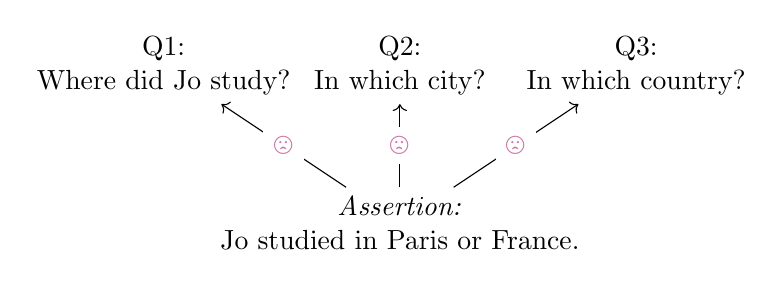
\begin{tikzpicture}
			\node[align=center] at(0, 0) (A) {\textit{Assertion:}\\ Jo studied in Paris or France.};
			\node[align=center] at(-3, 2) (Q1) {Q1:\\ Where did Jo study?};
			\node[align=center] at(0, 2) (Q2) {Q2:\\ In which city?};
			\node[align=center] at(3, 2) (Q3) {Q3:\\ In which country?};
			\draw[->] (A) -- (Q1) node[midway, fill=white] {\textcolor{red}{\frownie}};
			\draw[->] (A) -- (Q2) node[midway, fill=white] {\textcolor{red}{\frownie}};
			\draw[->] (A) -- (Q3) node[midway, fill=white] {\textcolor{red}{\frownie}};
		\end{tikzpicture}
	\end{center}
	
\end{frame}



\begin{frame}{Assertions and their implicit questions}
	\begin{itemize}
		\item What are questions ``compatible'' with assertions?
		\item Let's consider the following interpretation of \textsc{Question-Answer Congruence}:
	\end{itemize}
	\begin{exe}
		\exp{ex:qa-congruence} {\textsc{Question-Answer Congruence. } A question evoked by an assertion can be derived from it by replacing the focus-bearing element (if any) with the relevant \textit{wh}-word, or by adding the ?-operator, turning the assertion into a polar question.}
	\end{exe}
	\begin{itemize}
		\item A sentence like \textit{Jo studied in Paris}, then evokes questions likes \textit{Did Jo study in Paris?}, \textit{Where did Jo study?}, or \textit{In which city did Jo study?}
	\end{itemize}
\end{frame}

\begin{frame}{Questions as trees}
	\begin{minipage}{.55\linewidth}
		\begin{itemize}
			\item We submit that implicit questions are evoked by sentences compositionally.
			\item We also take question to be trees (=recursive partitions) instead of partitions.
			\item This allows for more expressivity, and more transparency between sentence structure and question structure.
		\end{itemize}
	\end{minipage}
	\hfill
	\begin{minipage}{.4\linewidth}
		\centering
		\begin{forest}
			[Jo studied in...[Europe[France[Paris][...]][Italy[...,roof]][...]][Asia[...,roof]][...]]
		\end{forest}
		\begin{forest}
			[Jo studied in...[Paris][not Paris]]
		\end{forest}
	\end{minipage}
\end{frame}

\begin{frame}{Flagging Questions Trees}
	\begin{itemize}
		\item When a simple assertion evokes an implicit question tree, leaves entailing the assertion get flagged.
		\item Negating an assertion flips the flags.
	\end{itemize}
	
	
	\begin{minipage}{.48\linewidth}
		\centering
		\scalebox{.8}{
			\begin{forest}
				[Jo studied in...[Europe[France[{Paris$^{\text{\faFlagCheckered}}$}][Lyon][...]][Italy[...,roof]][...]][Asia[...,roof]][...]]
		\end{forest}}
	\end{minipage}
	\hfill
	\begin{minipage}{.48\linewidth}
		\centering
		\scalebox{.8}{
			\begin{forest}
				[Jo studied in...[Europe[France[{Paris}][{Lyon$^{\text{\faFlagCheckered}}$}][{...$^{\text{\faFlagCheckered}}$}]][Italy[{...$^{\text{\faFlagCheckered}}$},roof]][...]][Asia[...,roof]][...]]
		\end{forest}}
	\end{minipage}
	\begin{itemize}
		\item What is the effect of complex operations, e.g. disjunctions and conditionals, on these trees? 
	\end{itemize}
\end{frame}

\begin{frame}{Disjoining Questions Trees}
	\begin{itemize}
		\item Disjunction merges the trees evoked by the disjuncts, retaining only those that are well-formed partitions.
	\end{itemize}
	\begin{minipage}{.27\linewidth}
		\centering
		\scalebox{.8}{
			\begin{forest}
				[Jo studied in...[France[{Paris$^{\text{\faFlagCheckered}}$}][Lyon][...]][Italy[...,roof]][...]]
		\end{forest}}
	\end{minipage}
	\hfill
	\begin{minipage}{.05\linewidth}
		\centering
		~\\~\\ \LARGE $\cup$
	\end{minipage}
	\hfill
	\begin{minipage}{.27\linewidth}
		\centering
		\scalebox{.8}{
			\begin{forest}
				[Jo studied in...[France[{Paris}][{Lyon$^{\text{\faFlagCheckered}}$}][...]][Italy[...,roof]][...]]
		\end{forest}}
	\end{minipage}
	\hfill
	\begin{minipage}{.05\linewidth}
		\centering
		~\\~\\ \LARGE $=$
	\end{minipage}
	\hfill
	\begin{minipage}{.27\linewidth}
		\centering
		\scalebox{.8}{
			\begin{forest}
				[Jo studied in...[France[{Paris$^{\text{\faFlagCheckered}}$}][{Lyon$^{\text{\faFlagCheckered}}$}][...]][Italy[...,roof]][...]]
		\end{forest}}
	\end{minipage}
\end{frame}

%\usebackgroundtemplate%
%{%
	%	\includegraphics[height=\paperwidth]{./giorno\_transparent.png}%
	%}
\begin{frame}
	\section[A Redundancy Case Study]{A Redundancy Case Study}
\end{frame}
\usebackgroundtemplate{}

\begin{frame}{A challenging dataset}
	\begin{itemize}
		\item ``Double'' disjunctions featuring the same disjunct twice are obviously odd.
	\end{itemize}
	\begin{exe}
		\ex[\#] {Jo studied in Paris, or in Paris or Lyon. \hfill $\p \vee (\p \vee \q)$}\label{ex:pvpvq}
	\end{exe}
	\begin{itemize}
		\item More intriguing is the contrast in (\ref{ex:redundancy-contrast}). (\ref{ex:pv(nptq)}) and (\ref{ex:pv(nqtp)}) can be both related to (\ref{ex:pvpvq}) \textit{via} the equivalence $\p \vee \q \equiv \neg \p \rightarrow \q \equiv \neg \q \rightarrow \p$; called \textit{or}-to-\textit{if} tautology.
	\end{itemize}
	\begin{exe}
		\ex \label{ex:redundancy-contrast}
		\begin{xlist}
			\ex[] {Jo studied in Paris, or if not in Paris then Lyon. \hfill $\p \vee (\neg \p \rightarrow \q)$}\label{ex:pv(nptq)}
			\ex[\#] {Jo studied in Paris, or if not in Lyon then Paris. \hfill $\p \vee (\neg \q \rightarrow \p)$}\label{ex:pv(nqtp)}
		\end{xlist}
	\end{exe}
	\begin{itemize}
		\item Earlier \textsc{Redundancy}-based approaches do not predict any contrast in (\ref{ex:redundancy-contrast}).\footnote{Other approaches do, but at the cost of mispredicting Hurford Disjunctions.}
	\end{itemize}
\end{frame}

\begin{frame}{Core Intuitions}
	
	\begin{exe}
		\exr{ex:pvpvq}[\#] {Jo studied in Paris, or in Paris or Lyon. \hfill $\p^{\text{\faFlagCheckered}} \vee (\p^{\text{\faFlagCheckered}} \vee \q)$}
		\exr{ex:redundancy-contrast}
		\begin{xlist}
			\ex[] {Jo studied in Paris, or if not in Paris then Lyon. \hfill $\p^{\text{\faFlagCheckered}} \vee (\neg \p \rightarrow \q)$}%\label{ex:pv(nptq)}
			\ex[\#] {Jo studied in Paris, or if not in Lyon then Paris. \hfill $\p^{\text{\faFlagCheckered}} \vee (\neg \q \rightarrow \p^{\text{\faFlagCheckered}})$}%\label{ex:pv(nqtp)}
		\end{xlist}
	\end{exe}
	\begin{itemize}
		\item The ``double'' disjunction in (\ref{ex:pvpvq}) flags \textit{Paris} twice: \textsc{Redundant}!
		\item In (\ref{ex:pv(nptq)}) \p's second occurrence is in the antecedent of a conditional: not flagged, so not \textsc{Redundant}!
		\item In (\ref{ex:pv(nqtp)}) \p's second occurrence is in the consequent of a conditional: \p{} gets flagged twice, so \textsc{Redundant}!
	\end{itemize}
\end{frame}

\begin{frame}{Q-Non-Redundancy}
	\begin{itemize}
		\item To capture the idea that multiple ``flagging'' is bad, we rephrase \textsc{Non-Redundancy} at the level of LF-question pairs.
	\end{itemize}
	\begin{exe}
		\ex {\textsc{Q-Non-Redundancy.} If an LF $X$ evokes a question-tree $T$, and a formal simplification of $X$ also evokes $T$ (flagged nodes included), then $T$ is odd given $X$.}
		\ex {\textsc{Sentence Oddness.} If any question-tree evoked by an LF $X$ is odd given $X$, then $X$ is odd \textit{simpliciter}.}
	\end{exe}
	\begin{itemize}
		\item The ``double'' disjunction in (\ref{ex:pvpvq}) is odd because whatever tree it evokes is evoked by $\p\vee\q$=\textit{Paris or Lyon}.
		\item (\ref{ex:pv(nptq)}) is \textit{not} odd because one of the trees it evokes is different from all the ones evoked by (\ref{ex:pv(nptq)})'s simplifications.
		\item In (\ref{ex:pv(nqtp)}) is odd, because whatever tree it evokes is evoked by $\p$=\textit{Paris}.
	\end{itemize}
\end{frame}
\begin{frame}{The ``double'' disjunction in (\ref{ex:pvpvq})}
	\begin{itemize}
		\item Recall questions evoked by disjunctions are well-formed unions of the disjuncts' question-trees.
		\item A question-tree for $\p\vee\q$ must then be about both \p and \q.
		\item Further disjoining with \p, does not do anything.
	\end{itemize}
	\begin{forest}
		[Jo studied in...[{Paris$^{\text{\faFlagCheckered}}$}][{Lyon}][...]]
	\end{forest}
	\begin{forest}
		[Jo studied in...[{Paris$^{\text{\faFlagCheckered}}$}][{Lyon$^{\text{\faFlagCheckered}}$}][...]]
	\end{forest}
	\begin{forest}
		[Jo studied in...[{Paris$^{\text{\faFlagCheckered}}$}][{Lyon$^{\text{\faFlagCheckered}}$}][...]]
	\end{forest}
	\begin{itemize}
		\item So, (\ref{ex:pvpvq})'s only question-tree, is also evoked by $\p\vee\q$, and thus (\ref{ex:pvpvq}) is odd due to \textsc{Q-Redundancy}.
	\end{itemize}
\end{frame}

\begin{frame}{The ``double'' disjunction in (\ref{ex:pvpvq})}
	\begin{itemize}
		\item Recall questions evoked by disjunctions are well-formed unions of the disjuncts' question-trees.
		\item A question-tree for $\p\vee\q$ must then be about both \p and \q.
		\item Further disjoining with \p, does not do anything.
	\end{itemize}
	\begin{forest}
		[Jo studied in...[{Paris$^{\text{\faFlagCheckered}}$}][{Lyon}][...]]
	\end{forest}
	\begin{forest}
		[Jo studied in...[{Paris$^{\text{\faFlagCheckered}}$}][{Lyon$^{\text{\faFlagCheckered}}$}][...]]
	\end{forest}
	\begin{forest}
		[Jo studied in...[{Paris$^{\text{\faFlagCheckered}}$}][{Lyon$^{\text{\faFlagCheckered}}$}][...]]
	\end{forest}
	\begin{itemize}
		\item So, (\ref{ex:pvpvq})'s only question-tree, is also evoked by $\p\vee\q$, and thus (\ref{ex:pvpvq}) is odd due to \textsc{Q-Redundancy}.
	\end{itemize}
\end{frame}



%\usebackgroundtemplate%
%{%
	%	\includegraphics[height=\paperwidth]{./jolyne\_transparent.png}%
	%}
\begin{frame}
	\section[Spooky action at a distance]{Spooky action at a distance}
\end{frame}
\usebackgroundtemplate{}

%\usebackgroundtemplate%
%{%
	%	\includegraphics[height=\paperwidth]{./johnny\_transparent.png}%
	%}
\begin{frame}
	\section[To Redundancy and Beyond]{To Redundancy and Beyond}
\end{frame}
\usebackgroundtemplate{}


\begin{frame}[allowframebreaks]{Selected references}
	\printbibliography[heading=none]
\end{frame}

\section{Appendix}


\end{document}